% ══════════════════════════════════════════════════════════════════════════════
% Standalone supplementary build.
%
% This is a thin wrapper that inputs sections/supplementary.tex, the same file
% that arxiv/main.tex uses for the supplement. There is exactly one source of
% truth for the supplementary content; edit sections/supplementary.tex.
% ══════════════════════════════════════════════════════════════════════════════

\documentclass[11pt]{article}

\usepackage[margin=1in]{geometry}
\usepackage{amsmath,amssymb,amsfonts}
\usepackage{graphicx}
\usepackage{booktabs}
\usepackage{hyperref}
\usepackage{xcolor}
\usepackage{caption}
\usepackage{subcaption}
\usepackage{placeins}

\graphicspath{{sections/figures/}}

\newcommand{\vxi}{\boldsymbol{\xi}}
\newcommand{\mhat}[1]{\hat{\mathbf{#1}}}
\newcommand{\R}{\mathbb{R}}
\newcommand{\norm}[1]{\left\lVert #1 \right\rVert}

\begin{document}

% ══════════════════════════════════════════════════════════════════════════════
% Supplementary Information
% ══════════════════════════════════════════════════════════════════════════════

% Reset counters for supplementary numbering
\setcounter{section}{0}
\setcounter{figure}{0}
\setcounter{table}{0}
\setcounter{equation}{0}
\renewcommand{\thesection}{S\arabic{section}}
\renewcommand{\thefigure}{S\arabic{figure}}
\renewcommand{\thetable}{S\arabic{table}}
\renewcommand{\theequation}{S\arabic{equation}}

\section*{Supplementary Information}

% ══════════════════════════════════════════════════════════════════════════════
\subsection*{Supplementary Tables}

% ── Table S1: Beta sweep ─────────────────────────────────────────────────
\begin{table}[ht]
\centering
\caption{\textbf{Inverse temperature sensitivity analysis.} SA generation
quality as a function of $\beta / \beta^*$, where $\beta^* \approx 2.94$ was
identified via entropy inflection in the 18-dimensional PCA space ($K{=}23$
stored patterns). Operating at $\beta = \beta^*$ (bold row) balances generation
novelty against fidelity. Med MRE = median relative error of per-feature means;
Novelty = $1 - \max_k \cos(\hat{\xi}, \hat{m}_k)$.}
\label{stab:beta-sweep}
\begin{tabular}{rrcccc}
\toprule
$\beta/\beta^*$ & $\beta$ & Noise scale & PC1 std ratio & Novelty & Med MRE (\%) \\
\midrule
0.1 & 0.29 & 0.261 & 0.538 & 0.542 & 0.7 \\
0.3 & 0.88 & 0.151 & 0.550 & 0.536 & 0.7 \\
0.5 & 1.47 & 0.117 & 0.562 & 0.528 & 0.7 \\
\textbf{1.0} & \textbf{2.94} & \textbf{0.082} & \textbf{0.589} & \textbf{0.502} & \textbf{0.6} \\
1.5 & 4.41 & 0.067 & 0.613 & 0.474 & 0.7 \\
2.0 & 5.88 & 0.058 & 0.638 & 0.446 & 0.7 \\
3.0 & 8.82 & 0.048 & 0.689 & 0.403 & 0.8 \\
\bottomrule
\end{tabular}
\end{table}

% ── Table S2: Multiplicity weighting parameters ─────────────────────────
\begin{table}[ht]
\centering
\caption{\textbf{Multiplicity weighting parameters for conditional generation.}
The multiplicity ratio $\rho$ was computed to achieve a target effective fraction
$f_{\text{target}} = 0.80$ of softmax attention on the designated patterns.
$K_{\text{eff}}$ is the participation ratio quantifying the effective number of
patterns contributing to generation.}
\label{stab:multiplicity}
\begin{tabular}{lccccc}
\toprule
Condition & $K_{\text{sub}}$ & $K_{\text{bg}}$ & $\rho$ & $f_{\text{eff}}$ & $K_{\text{eff}}$ \\
\midrule
Uncomplicated  & 18 & 5  & 1.11  & 0.80 & 23.0 \\
PCOS           & 3  & 20 & 26.67 & 0.80 & 4.6 \\
Developed PE   & 5  & 18 & 14.40 & 0.80 & 7.7 \\
\bottomrule
\end{tabular}
\end{table}

% ── Table S3: SA Hyperparameters ─────────────────────────────────────────
\begin{table}[ht]
\centering
\caption{\textbf{SA generation hyperparameters.} The same values were used for
unconditioned and conditioned generation except where noted.}
\label{stab:hyperparams}
\begin{tabular}{lll}
\toprule
Parameter & Value & Description \\
\midrule
$\alpha$ & 0.01 & Langevin step size (see Table~\ref{tab:ula-vs-mala}) \\
$T$ & 2,000 & Langevin iterations per sample \\
$\beta^*$ & 2.94 & Inverse temperature (entropy inflection) \\
PCA threshold & 95\% & Variance retained \\
$d_{\text{PCA}}$ & 18 & PCA dimensionality \\
$N$ & 100 & Synthetic patients per cohort \\
Random seed & 42 & For reproducibility \\
$f_{\text{target}}$ & 0.80 & Target attention fraction (conditioned only) \\
\bottomrule
\end{tabular}
\end{table}

% ── Table S4: ODE Calibration Details ────────────────────────────────────
\begin{table}[ht]
\centering
\caption{\textbf{BZ2012 ODE model calibration.} Five rate constants were
calibrated on Visit~1 real patients ($n{=}23$) using bounded Nelder--Mead
optimization in log-scale-factor space. The cost function was the mean
normalized relative squared error across five TGA features under TF-only
conditions. Bounds: $\pm\log(100)$. Convergence: $f_{\text{tol}} = 10^{-6}$,
500 iterations, 11 random restarts.}
\label{stab:ode-calibration}
\begin{tabular}{llrrl}
\toprule
Rate constant & Role & Default & Calibrated & Scale \\
\midrule
prothrombinase $k_{\text{cat}}$ & Thrombin burst & 63.5 s$^{-1}$ & 21.94 s$^{-1}$ & 0.35$\times$ \\
intrinsic Xase $k_{\text{cat}}$ & Amplification Xa & 8.2 s$^{-1}$ & 0.169 s$^{-1}$ & 0.021$\times$ \\
extrinsic Xase $k_{\text{cat}}$ & Initiation Xa & 6.0 s$^{-1}$ & 93.2 s$^{-1}$ & 15.5$\times$ \\
PC activation $k_{\text{cat}}$ & Protein C activation & 0.41 s$^{-1}$ & 0.890 s$^{-1}$ & 2.17$\times$ \\
mIIa conversion $k$ & mIIa$\to$IIa & $2.3{\times}10^8$ & $1.15{\times}10^9$ & 5.01$\times$ \\
\bottomrule
\multicolumn{5}{l}{\small Units for mIIa conversion: M$^{-1}$s$^{-1}$} \\
\end{tabular}
\end{table}

% ── Table S5: Full MRE summary ───────────────────────────────────────────
\begin{table}[ht]
\centering
\caption{\textbf{Summary of mean relative errors across all 72 features.}
Per-visit distribution of MREs between real and SA-generated synthetic patient
means. The full feature-by-feature table (72 features $\times$ 3 visits = 216
entries) is provided in the code repository as
\texttt{paper\_summary\_statistics.csv}.}
\label{stab:mre-summary}
\begin{tabular}{lcccccc}
\toprule
Visit & Median MRE & Mean MRE & 25th pctl & 75th pctl & Max MRE & Below 5\% \\
\midrule
V1 (baseline)   & 0.022 & 0.029 & 0.008 & 0.039 & 0.158 & 59/72 (81.9\%) \\
V2 (1st tri)    & 0.009 & 0.021 & 0.004 & 0.022 & 0.224 & 65/72 (90.3\%) \\
V3 (3rd tri)    & 0.011 & 0.016 & 0.005 & 0.024 & 0.062 & 69/72 (95.8\%) \\
\midrule
\textbf{Pooled (all 3 visits)} & \textbf{0.012} & \textbf{0.022} & \textbf{0.005} & \textbf{0.028} & \textbf{0.224} & \textbf{193/216 (89.4\%)} \\
\bottomrule
\multicolumn{7}{p{0.95\textwidth}}{\small Pooled median MRE 95\% bootstrap CI: (0.98\%, 1.60\%) over 10{,}000 resamples (seed~42).}
\end{tabular}
\end{table}

% ── Table S6: CTGAN/TVAE comparison ──────────────────────────────────────
\begin{table}[ht]
\centering
\caption{\textbf{Comparison with deep generative baselines.} CTGAN and TVAE
were trained on the same 90 per-visit records (23 patients $\times$ 3 visits,
72 features) at three epoch counts. SA and MVN results from the main text are
shown for reference. CTGAN fails at this sample size (median MRE
$\approx$~19\%), consistent with GAN mode collapse on small datasets. TVAE
achieves comparable marginal fidelity at high epoch counts but cannot capture
cross-visit covariance or perform conditional generation.}
\label{stab:ctgan}
\begin{tabular}{lcccc}
\toprule
Method & Epochs & Med MRE & Med KS & Corr MAE \\
\midrule
SA              & --   & 0.019 & 0.169 & 0.200 \\
MVN             & --   & 0.024 & 0.161 & 0.090 \\
\midrule
CTGAN           & 300   & 0.189 & 0.364 & 0.261 \\
CTGAN           & 1,000 & 0.195 & 0.349 & 0.265 \\
CTGAN           & 3,000 & 0.187 & 0.341 & 0.180 \\
\midrule
TVAE            & 300   & 0.037 & 0.174 & 0.152 \\
TVAE            & 1,000 & 0.026 & 0.248 & 0.082 \\
TVAE            & 3,000 & 0.018 & 0.224 & 0.092 \\
\bottomrule
\end{tabular}
\end{table}

% ── Table S7: PCA sensitivity ────────────────────────────────────────────
\begin{table}[ht]
\centering
\caption{\textbf{PCA variance threshold sensitivity analysis.} SA generation
quality is stable across thresholds from 85\% to 99\%. Median MRE remains
between 1.0\% and 1.7\% across all thresholds. The 95\% threshold used in the
main text (bold) is not a critical design choice.}
\label{stab:pca-sensitivity}
\begin{tabular}{rrccccc}
\toprule
Threshold & $d_{\text{PCA}}$ & $K/d$ & $\beta^*$ & Novelty & Med MRE & Corr MAE \\
\midrule
85\% & 13 & 1.77 & 2.94 & 0.420 & 0.0098 & 0.124 \\
90\% & 15 & 1.53 & 2.94 & 0.477 & 0.0160 & 0.126 \\
\textbf{95\%} & \textbf{18} & \textbf{1.28} & \textbf{2.94} & \textbf{0.500} & \textbf{0.0124} & \textbf{0.143} \\
97.5\% & 20 & 1.15 & 2.94 & 0.543 & 0.0120 & 0.135 \\
99\% & 21 & 1.10 & 2.94 & 0.541 & 0.0172 & 0.138 \\
\bottomrule
\end{tabular}
\end{table}

% ── Table S8: ULA vs MALA diagnostics ──────────────────────────────────
\begin{table}[ht]
\centering
\caption{\textbf{ULA vs MALA sampling diagnostics.} Ten chains of 5{,}000
iterations each were run with both the Unadjusted Langevin Algorithm (ULA)
and the Metropolis-Adjusted Langevin Algorithm (MALA) at step size
$\alpha = 0.01$ and $\beta^* = 2.94$ on the 18-dimensional PCA memory
($K{=}23$ patterns). The MALA acceptance rate of $99.9\%$ confirms that
virtually every ULA proposal satisfies detailed balance, and the
indistinguishable energy and effective sample size statistics confirm
negligible discretization bias. \rone{This comparison bounds the
discretization error of the reported sampler. The direct reference for the
target itself is the analytic sampler of Eq.~\maineqref{eq:exact_mixture},
introduced below.}}
\label{tab:ula-vs-mala}
\begin{tabular}{lcc}
\toprule
Metric & ULA & MALA \\
\midrule
Acceptance rate (\%)         & -- (no rejection) & $99.9 \pm 0.03$ \\
Mean energy (post-burn-in)   & $1.932 \pm 0.141$ & $1.886 \pm 0.231$ \\
$\tau_{\text{int}}$          & $109.5 \pm 49.5$  & $106.7 \pm 30.4$ \\
Effective sample size        & $41.8 \pm 14.2$   & $40.0 \pm 10.2$ \\
\bottomrule
\multicolumn{3}{p{0.85\textwidth}}{\small Burn-in: 1{,}000 iterations discarded. $\tau_{\text{int}}$: integrated
autocorrelation time estimated with a windowed estimator (threshold 0.05).
ESS = $(T - T_{\text{burn}}) / \tau_{\text{int}}$.}
\end{tabular}
\end{table}

% ── Table S9: Memorization diagnostics ─────────────────────────────────
\begin{table}[ht]
\centering
\caption{\textbf{Memorization diagnostics.} Two complementary checks that
SA-generated patients are not memorized copies of the $K{=}23$ stored profiles.
Novelty score is the angular distance between a synthetic sample and its
nearest stored pattern at $\beta = \beta^*$. Nearest-neighbor distances are
computed in the per-visit standardized 72-dimensional feature space.}
\label{stab:memorization}
\begin{tabular}{lc}
\toprule
Metric & Value \\
\midrule
Mean novelty score, $1 - \max_k \cos(\hat{\xi}, \hat{m}_k)$ & 0.50 \\
Median synth--real nearest-neighbor distance (std.\ units) & 6.14 \\
Median real--real nearest-neighbor distance (std.\ units)  & 6.87 \\
Distance ratio (synth--real / real--real)                  & 0.89 \\
\bottomrule
\end{tabular}
\end{table}

% ── Table S10: Bootstrap MW per feature × condition ───────────────────
\begin{table}[ht]
\centering
\caption{\textbf{Bootstrap Mann--Whitney equivalence per feature and
condition.} For each of 24 feature--condition pairs, we subsampled the
synthetic cohort to match the real sample size, applied a Mann--Whitney U test,
and repeated 1{,}000 times. Frac.\ $p > 0.05$ is the fraction of replicates in
which the test could not distinguish the synthetic from the real distribution.
20 of 24 pairs achieve $p > 0.05$ in $\geq 90\%$ of replicates; the four
failing pairs (italicized) all involve high-variance features in the smallest
subgroups.}
\label{stab:bootstrap-mw}
\begin{tabular}{llcc}
\toprule
Condition & Feature & MRE & Frac.\ $p > 0.05$ \\
\midrule
Uncomplicated ($n{=}18$) & FVIII   & 0.057 & 0.952 \\
Uncomplicated ($n{=}18$) & vWF     & 0.022 & 0.999 \\
Uncomplicated ($n{=}18$) & FIX     & 0.018 & 0.998 \\
Uncomplicated ($n{=}18$) & FV      & 0.006 & 0.996 \\
Uncomplicated ($n{=}18$) & $\alpha_2$-AP & 0.019 & 1.000 \\
Uncomplicated ($n{=}18$) & FVII    & 0.057 & 0.941 \\
Uncomplicated ($n{=}18$) & Fbgn    & 0.017 & 0.987 \\
Uncomplicated ($n{=}18$) & Plgn    & 0.020 & 0.988 \\
\midrule
PCOS ($n{=}3$)  & FVIII   & 0.109 & 0.985 \\
PCOS ($n{=}3$)  & vWF     & 0.150 & 0.959 \\
PCOS ($n{=}3$)  & \textit{FIX}     & \textit{0.121} & \textit{0.873} \\
PCOS ($n{=}3$)  & FV      & 0.057 & 0.944 \\
PCOS ($n{=}3$)  & $\alpha_2$-AP & 0.051 & 0.987 \\
PCOS ($n{=}3$)  & FVII    & 0.029 & 0.999 \\
PCOS ($n{=}3$)  & Fbgn    & 0.043 & 0.992 \\
PCOS ($n{=}3$)  & \textit{Plgn}    & \textit{0.153} & \textit{0.615} \\
\midrule
Developed PE ($n{=}5$) & FVIII   & 0.097 & 0.932 \\
Developed PE ($n{=}5$) & vWF     & 0.010 & 0.986 \\
Developed PE ($n{=}5$) & \textit{FIX}     & \textit{0.108} & \textit{0.780} \\
Developed PE ($n{=}5$) & FV      & 0.006 & 0.987 \\
Developed PE ($n{=}5$) & $\alpha_2$-AP & 0.062 & 0.950 \\
Developed PE ($n{=}5$) & FVII    & 0.045 & 0.993 \\
Developed PE ($n{=}5$) & Fbgn    & 0.048 & 0.996 \\
Developed PE ($n{=}5$) & \textit{Plgn}    & \textit{0.093} & \textit{0.814} \\
\bottomrule
\multicolumn{4}{p{0.95\textwidth}}{\small Median Frac.\ $p > 0.05$ across all 24 pairs: 0.986. Failing
pairs ($< 0.90$, italicized): PCOS--FIX, PCOS--Plgn, DPE--FIX, DPE--Plgn.}
\end{tabular}
\end{table}

% ── Table S11: Mechanistic validation diagnostics ─────────────────────
\begin{table}[ht]
\centering
\caption{\textbf{Mechanistic validation diagnostics per feature and
condition.} Cloud overlap is the fraction of synthetic ODE-predicted/measured
ratios falling within the 5th--95th percentile of the corresponding real
distribution. KS $D$ and KS $p$ are from a two-sample Kolmogorov--Smirnov test
on the same ratio distributions. Real $n{=}69$ (23 patients $\times$ 3 visits);
synthetic $n{=}300$ (100 patients $\times$ 3 visits).}
\label{stab:mechanistic-validation}
\begin{tabular}{llccc}
\toprule
Condition & TGA Feature & Cloud overlap & KS $D$ & KS $p$ \\
\midrule
TF-only & Lagtime          & \rone{0.92} & 0.112 & \rone{0.48} \\
TF-only & Peak             & \rone{0.91} & 0.081 & \rone{0.86} \\
TF-only & T.Peak           & \rone{0.92} & 0.102 & \rone{0.61} \\
TF-only & Max Rate         & \rone{0.91} & 0.083 & \rone{0.84} \\
TF-only & ETP              & \rone{0.83} & 0.123 & \rone{0.36} \\
\midrule
TF+TM   & Lagtime          & \rone{0.92} & 0.127 & \rone{0.32} \\
TF+TM   & Peak             & \rone{0.88} & 0.079 & \rone{0.88} \\
TF+TM   & T.Peak           & \rone{0.91} & 0.110 & \rone{0.51} \\
TF+TM   & Max Rate         & \rone{0.88} & 0.096 & \rone{0.67} \\
TF+TM   & ETP              & \rone{0.89} & 0.112 & \rone{0.48} \\
\bottomrule
\multicolumn{5}{p{0.95\textwidth}}{\small \rone{TF-only cloud overlap range: 0.83--0.92. TF+TM
cloud overlap range: 0.88--0.92. Pooled across both conditions and all five features, 0.902.}
KS $D$ range across both conditions: 0.079--0.127, all $p > 0.30$.}
\end{tabular}
\end{table}

% ── Table S12: Downstream utility per feature ─────────────────────────
\begin{table}[ht]
\centering
\caption{\textbf{Downstream utility — per-feature held-out V2/V3 performance.}
Median relative error of the BZ2012 ODE-predicted TGA values against the held-out
real V2 and V3 measurements, for the model calibrated on real V1 patients
($K{=}23$) and the model calibrated on synthetic V1 patients ($N{=}100$). The
synth-calibrated model achieves slightly lower error on every feature. Synth/Real
ratio $< 1$ favors the synth-calibrated model.}
\label{stab:downstream-utility}
\begin{tabular}{lccc}
\toprule
TGA Feature & Real-cal MRE & Synth-cal MRE & Synth/Real \\
\midrule
Lagtime           & 0.165 & 0.162 & 0.98$\times$ \\
Peak              & 0.097 & 0.087 & 0.90$\times$ \\
T.Peak            & 0.330 & 0.306 & 0.93$\times$ \\
Max Rate          & 0.286 & 0.259 & 0.91$\times$ \\
ETP               & 0.197 & 0.183 & 0.93$\times$ \\
\midrule
\textbf{Overall median} & \textbf{0.201} & \textbf{0.189} & \textbf{0.94$\times$} \\
\bottomrule
\end{tabular}
\end{table}

% ── Table S8: PCA-space ablation (E1) ────────────────────────────────────
\begin{table}[ht]
\centering
\caption{\rone{\textbf{PCA-space ablation.} Five generators fit in the identical
$d{=}18$ PCA subspace and evaluated on the same harness as SA. Median relative error
(MRE) and the mechanistic cloud overlap measure fidelity. Median novelty measures distance
from the stored patterns, and Frac.\ novel is the fraction above the $0.2$ novelty threshold.
The cross-visit Frobenius error is the deviation of the synthetic correlation matrix from the
real one. A lower value means staying closer to the $23$ real patients, so this metric
rewards memorization. The shared subspace is necessary but not sufficient.
$k$-nearest-neighbor interpolation collapses novelty, and the kernel-density estimator
degrades marginal and mechanistic fidelity, despite both being fit in it. The mixture and
copula baselines match SA on the fidelity axes.}}
\label{stab:pca-ablation}
\begin{tabular}{lccccc}
\toprule
Method & MRE (\%) & Cross-visit Frob. & Mech.\ overlap & Median novelty & Frac.\ novel \\
\midrule
SA         & 1.24 & 0.641 & 0.902 & 0.514 & 1.00 \\
PCA+GMM    & 1.13 & 0.422 & 0.918 & 0.497 & 0.94 \\
PCA+KDE    & 1.94 & 0.337 & 0.823 & 0.249 & 0.65 \\
PCA+kNN    & 1.63 & 0.587 & 0.938 & 0.051 & 0.05 \\
PCA+Copula & 1.34 & 0.417 & 0.934 & 0.462 & 1.00 \\
\bottomrule
\end{tabular}
\end{table}

% ── Table S9: convex-hull geometry (E2) ──────────────────────────────────
\begin{table}[ht]
\centering
\caption{\rtwo{\textbf{Convex-hull membership does not discriminate at $K{=}23$ in
$d{=}18$.} Hull membership and distance for the $100$ synthetic patients against the $23$
real patients, and for each real patient against the other $22$. The radial factor $t^{*}$
is where the ray from the hull centroid through a point exits the hull, so $1/t^{*}$ is the
factor by which a point overshoots the boundary and $t^{*} \ge 1$ would mean the point is
inside. Distances and overshoots are severity-matched, with each point's nearest vertex
removed on both sides, because a held-out real patient necessarily loses its own vertex.
Matched this way, the distance to the hull is not distinguishable between synthetic and real
patients (Mann--Whitney $p = 0.07$), while the radial overshoot is smaller for the synthetic
ones ($p < 10^{-4}$). Both tests treat the $100$ synthetic patients as independent, which
they are not, so the reported significance is optimistic. The geometry rows show why no point
of either kind falls inside. The hull attains the patients' typical radius only along the
$23$ vertex directions, and the sampler returns every sample to the unit sphere. A point
inside the hull of unit-norm patterns would have to be one of those patterns.}}
\label{stab:hull-geometry}
\begin{tabular}{lcc}
\toprule
Quantity & Synthetic ($n{=}100$) & Real, leave-one-out ($n{=}23$) \\
\midrule
Fraction inside hull                        & $0.00$ & $0.00$ \\
Median distance to hull                     & $11.0$ & $11.9$ \\
Median radial overshoot $1/t^{*}$           & $10.5$ & $15.2$ \\
\midrule
\multicolumn{3}{l}{\emph{Hull geometry of the real cohort}} \\
Median patient radius                       & \multicolumn{2}{c}{$13.8$} \\
Median hull extent, generic direction       & \multicolumn{2}{c}{$2.0$} \\
Largest $t^{*}$ attained on the unit sphere & \multicolumn{2}{c}{$0.231$} \\
\midrule
\multicolumn{3}{l}{\emph{Plausibility of the out-of-hull synthetic patients}} \\
Biological constraints satisfied            & \multicolumn{2}{c}{$81/100$} \\
Mechanistic band, per feature               & \multicolumn{2}{c}{$83$ to $92\%$} \\
Mechanistic band, all features and visits   & \multicolumn{2}{c}{$41/100$} \\
\bottomrule
\end{tabular}
\end{table}

% ── Table S10: membership-inference decomposition (E3) ───────────────────
\begin{table}[ht]
\centering
\caption{\rone{\textbf{Membership inference recovers memory membership, not unseen
patients.} Median nearest-neighbor distances in the standardized $216$-dimensional space,
and the attack's discrimination. The attack retrains the generator on $15$ training
patients and scores each real record by its distance to the resulting synthetic set,
treating the $15$ training patients as members and the $8$ held-out patients as
non-members. Every quantity comes from the same protocol. We drew $40$ partitions at random
with the generation seed held fixed, so that only the partition varies, and pooled the
distances across all partitions. Non-members sit at the same distance from the synthetic
cohort as unrelated real patients sit from one another. The synthetic cohort
carries no proximity signal about patients the generator never saw, and the discrimination
comes entirely from members sitting closer.}}
\label{stab:membership}
\begin{tabular}{lc}
\toprule
Quantity & Value \\
\midrule
\multicolumn{2}{l}{\emph{Median nearest-neighbor distance}} \\
Training member to nearest synthetic           & $10.7$ \\
Held-out non-member to nearest synthetic       & $15.4$ \\
Real to nearest real, leave-one-out            & $15.9$ \\
Synthetic to nearest real                      & $13.8$ \\
\midrule
\multicolumn{2}{l}{\emph{Membership-inference AUC over $40$ random splits}} \\
Mean                                           & $0.97$ \\
Standard deviation                             & $0.02$ \\
Median                                         & $0.98$ \\
Minimum                                        & $0.90$ \\
Maximum                                        & $1.00$ \\
Splits reaching perfect separation             & $9/40$ \\
Splits with AUC above $0.9$                    & $39/40$ \\
\bottomrule
\end{tabular}
\end{table}

\FloatBarrier

% ══════════════════════════════════════════════════════════════════════════════
\subsection*{Supplementary Figures}

% ── Fig S1: Cross-visit corr amplified ───────────────────────────────────
\begin{figure}[ht]
\centering
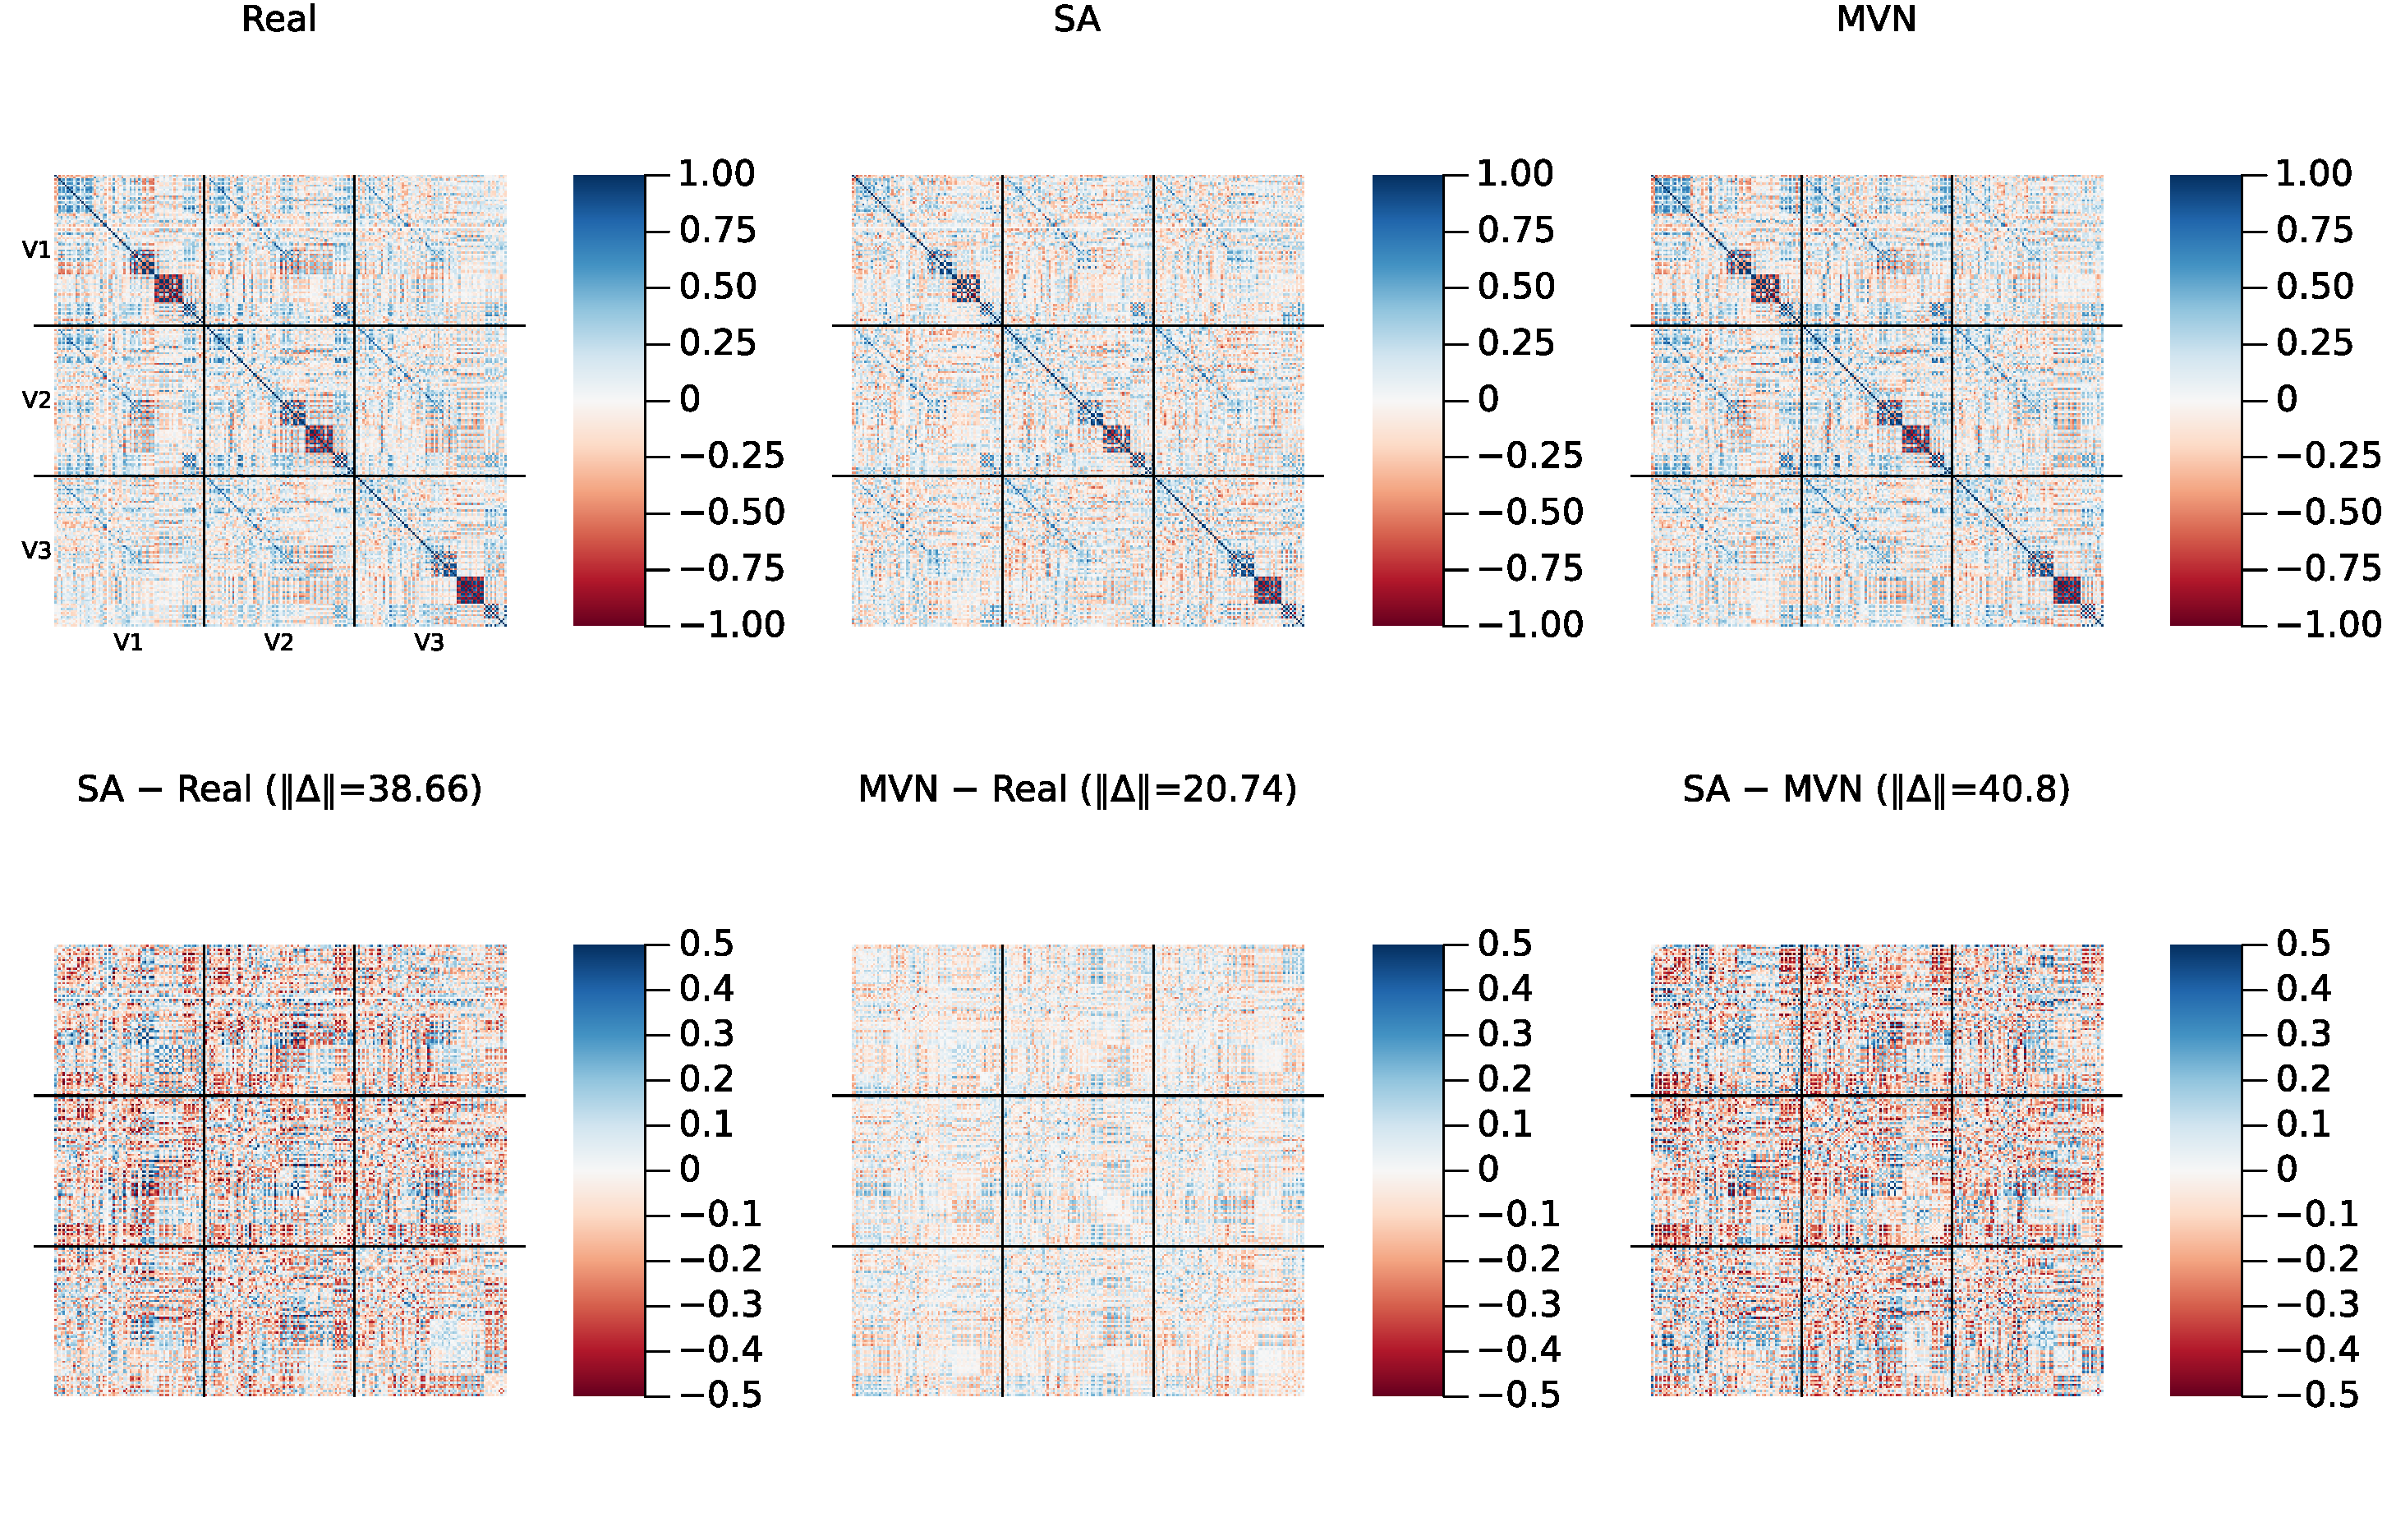
\includegraphics[width=\textwidth]{validate_cross_visit_corr_supp.pdf}
\caption{\textbf{Cross-visit correlation structure (amplified residual scale).}
Same layout as the main-text correlation figure, but with the bottom-row
residual panels plotted on a $\pm 0.5$ color scale (vs.\ $\pm 1.0$ in the main
text) to reveal fine structure. Frobenius norms of each residual matrix are
shown in the panel titles.}
\label{sfig:cross-visit-corr-supp}
\end{figure}

% ── Fig S2: Eigenvalue spectrum ──────────────────────────────────────────
\begin{figure}[ht]
\centering
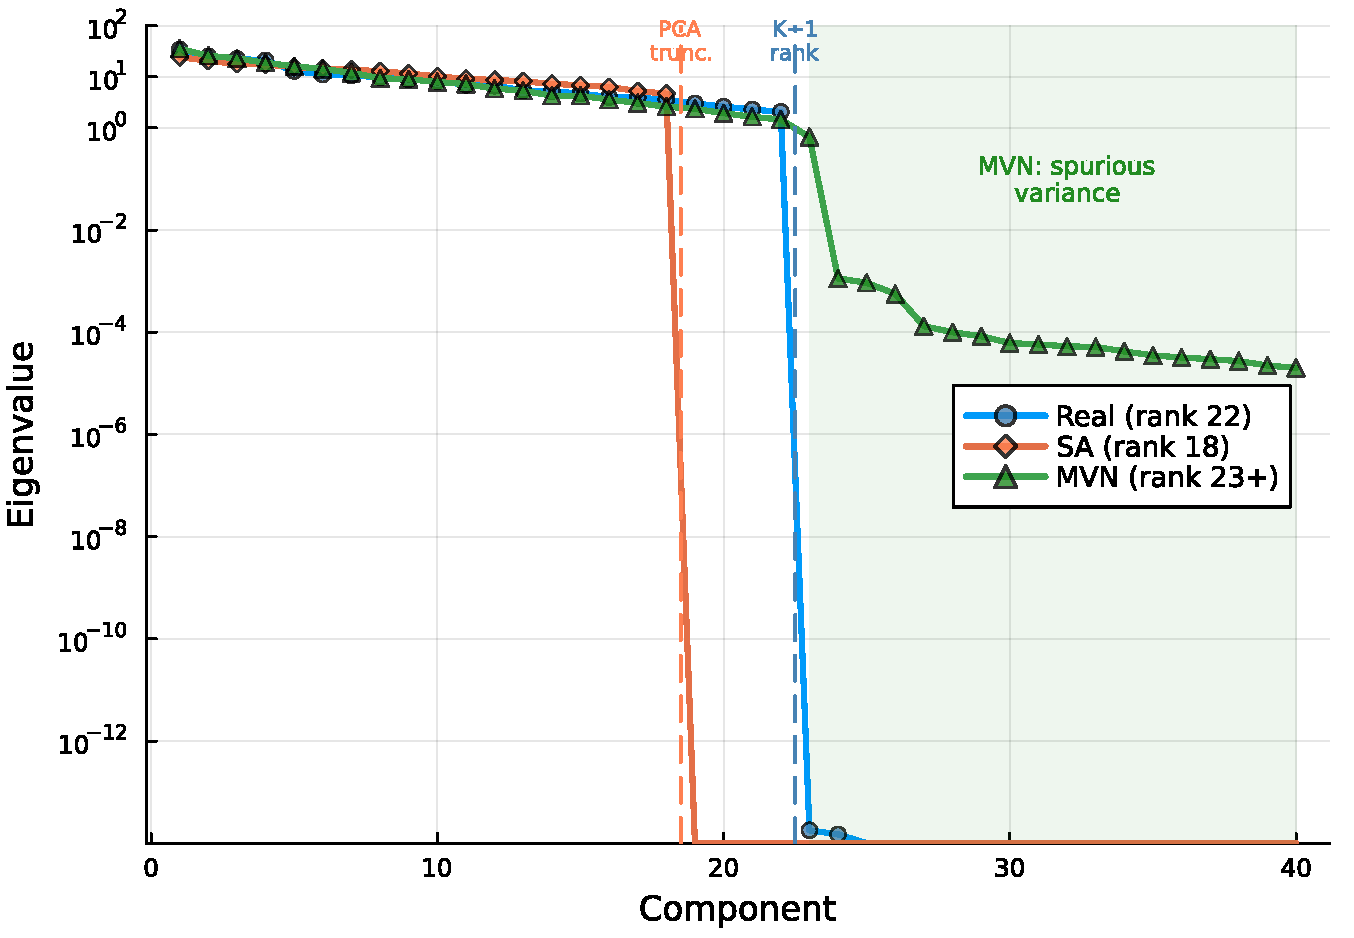
\includegraphics[width=0.75\textwidth]{validate_eigenvalue_spectrum.pdf}
\caption{\textbf{Covariance eigenvalue spectrum.} Log-scale eigenvalues of the
$216 \times 216$ sample covariance for Real ($K{=}23$, rank~22), SA ($N{=}100$,
rank~18), and MVN ($N{=}100$) populations. Dashed vertical lines mark the SA
PCA truncation point (component~18) and the data rank limit (component~22).
MVN's Ledoit--Wolf regularization inflates eigenvalues beyond component~22
(green shaded region), introducing spurious variance in 194 dimensions where the
data contain no signal.}
\label{sfig:eigenvalue-spectrum}
\end{figure}

% ── Fig S3: Conditioned generation PCA (pooled) ─────────────────────────
\begin{figure}[ht]
\centering

\includegraphics[width=0.65\textwidth]{validate_conditioned_pca.pdf}
\caption{\textbf{Conditioned generation: PCA projection (pooled).} Large
markers: real patients (blue = Uncomplicated, $n{=}18$; orange = PCOS, $n{=}3$;
red = Developed~PE, $n{=}5$). Small markers: synthetic patients ($N{=}100$ per
condition). With only 3 PCOS and 5 Developed~PE patients, the subgroups do not form
clearly separable clusters in the first two principal components, but the
synthetic cohorts concentrate around their respective real counterparts.}
\label{sfig:conditioned-pca}
\end{figure}

% ── Fig S4: Conditioned generation by visit ──────────────────────────────
\begin{figure}[ht]
\centering

\includegraphics[width=\textwidth]{validate_conditioned_pca_by_visit.pdf}
\caption{\textbf{Conditioned generation: PCA projection by visit.} Same as
Fig.~\ref{sfig:conditioned-pca} but separated by visit (V1, V2,
V3). Condition-specific clustering is maintained within each individual visit.}
\label{sfig:conditioned-by-visit}
\end{figure}

% ── Fig S5: Mechanistic TF+TM (combined scatter + ratios) ───────────────
\begin{figure}[ht]
\centering
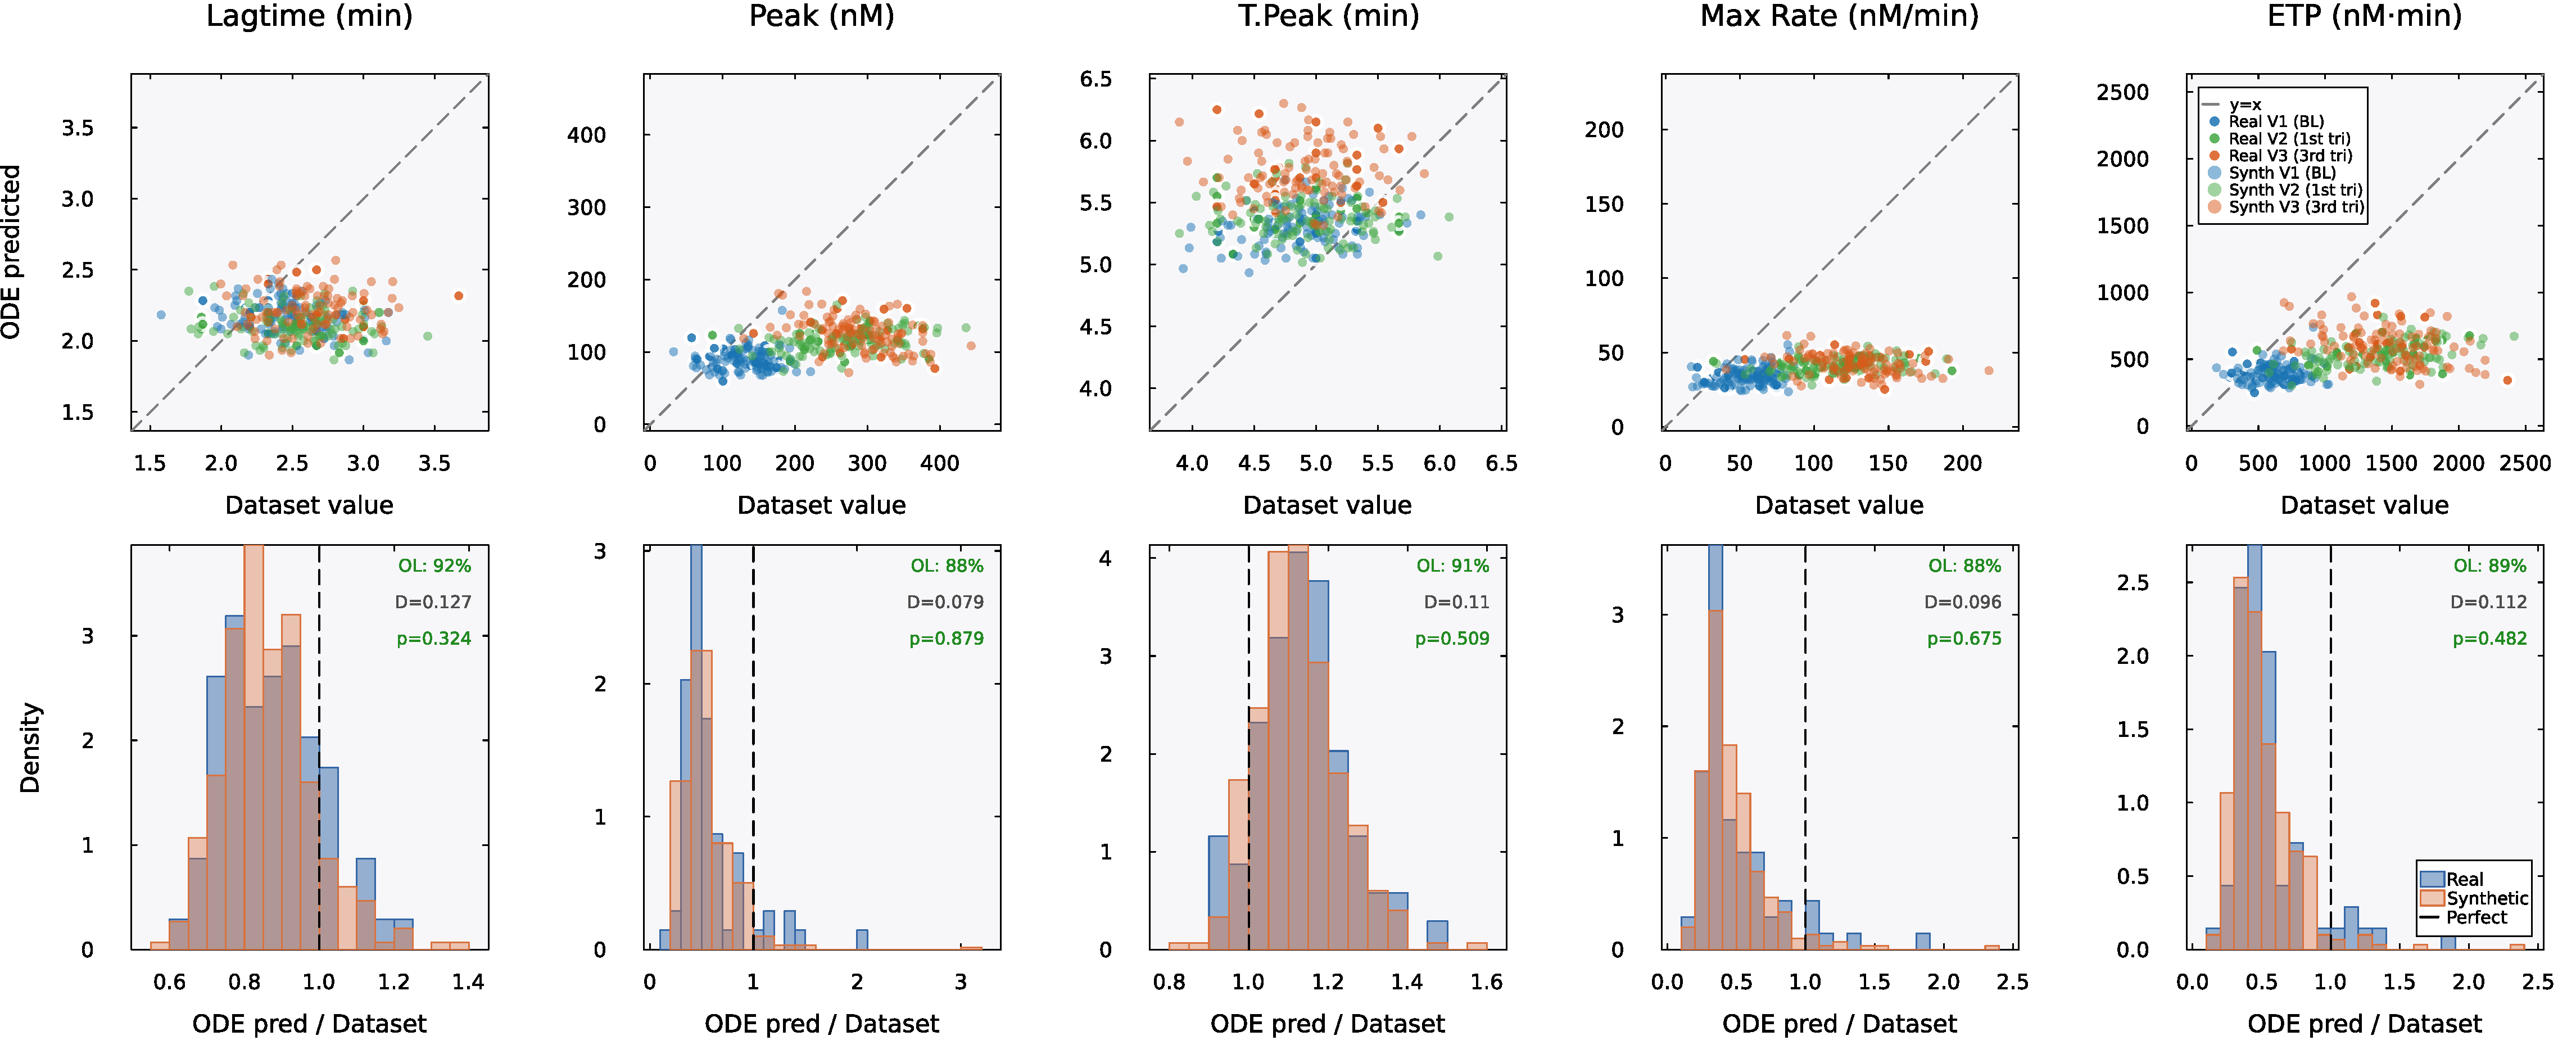
\includegraphics[width=\textwidth]{validate_mechanistic_combined_tf_tm_v2.pdf}
\caption{\textbf{Mechanistic validation (TF+TM condition).} Same layout as
main-text Fig.~6 but under TF+TM conditions. The model systematically
underpredicts peak and maximum rate ($\approx 0.5\times$ measured) for both
real and synthetic patients, reflecting overcorrection of the protein~C
anticoagulant pathway. Cloud overlap remains high at 88--92\%, confirming that
the model processes real and synthetic patients identically even under imperfect
calibration conditions.}
\label{sfig:mechanistic-tm-combined}
\end{figure}

% ── Fig S6: Cross-visit generalization (TF-only + TF+TM) ────────────────
\begin{figure}[ht]
\centering
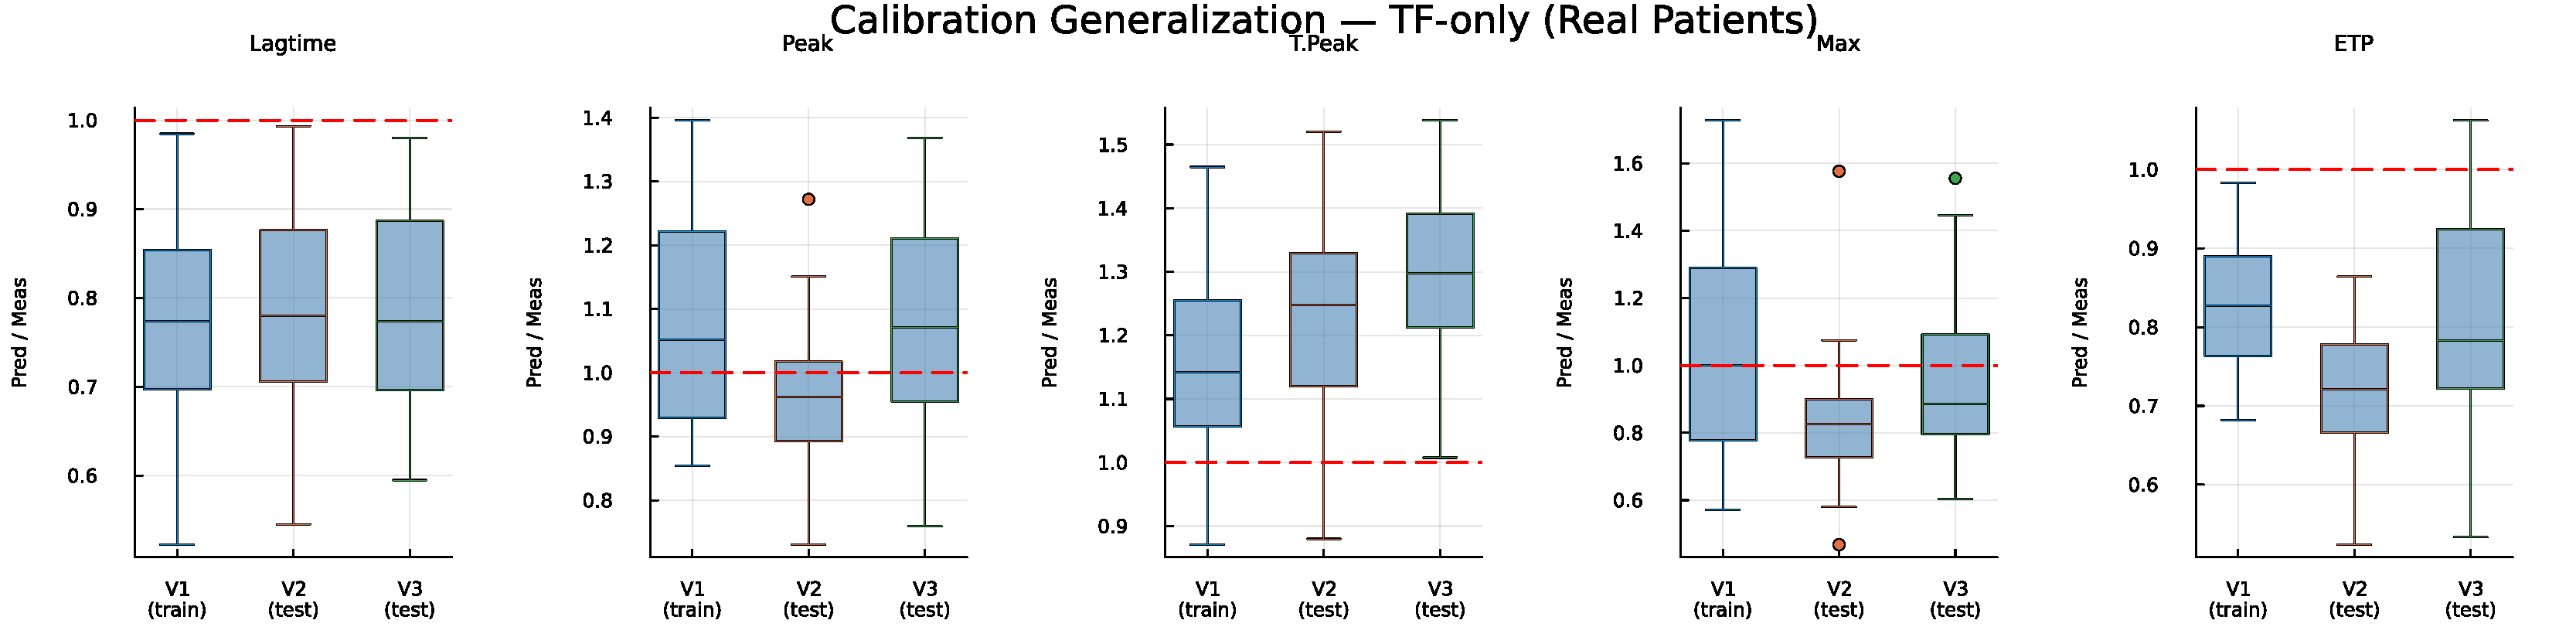
\includegraphics[width=\textwidth]{validate_mechanistic_generalization_tf_only.pdf}\\[6pt]
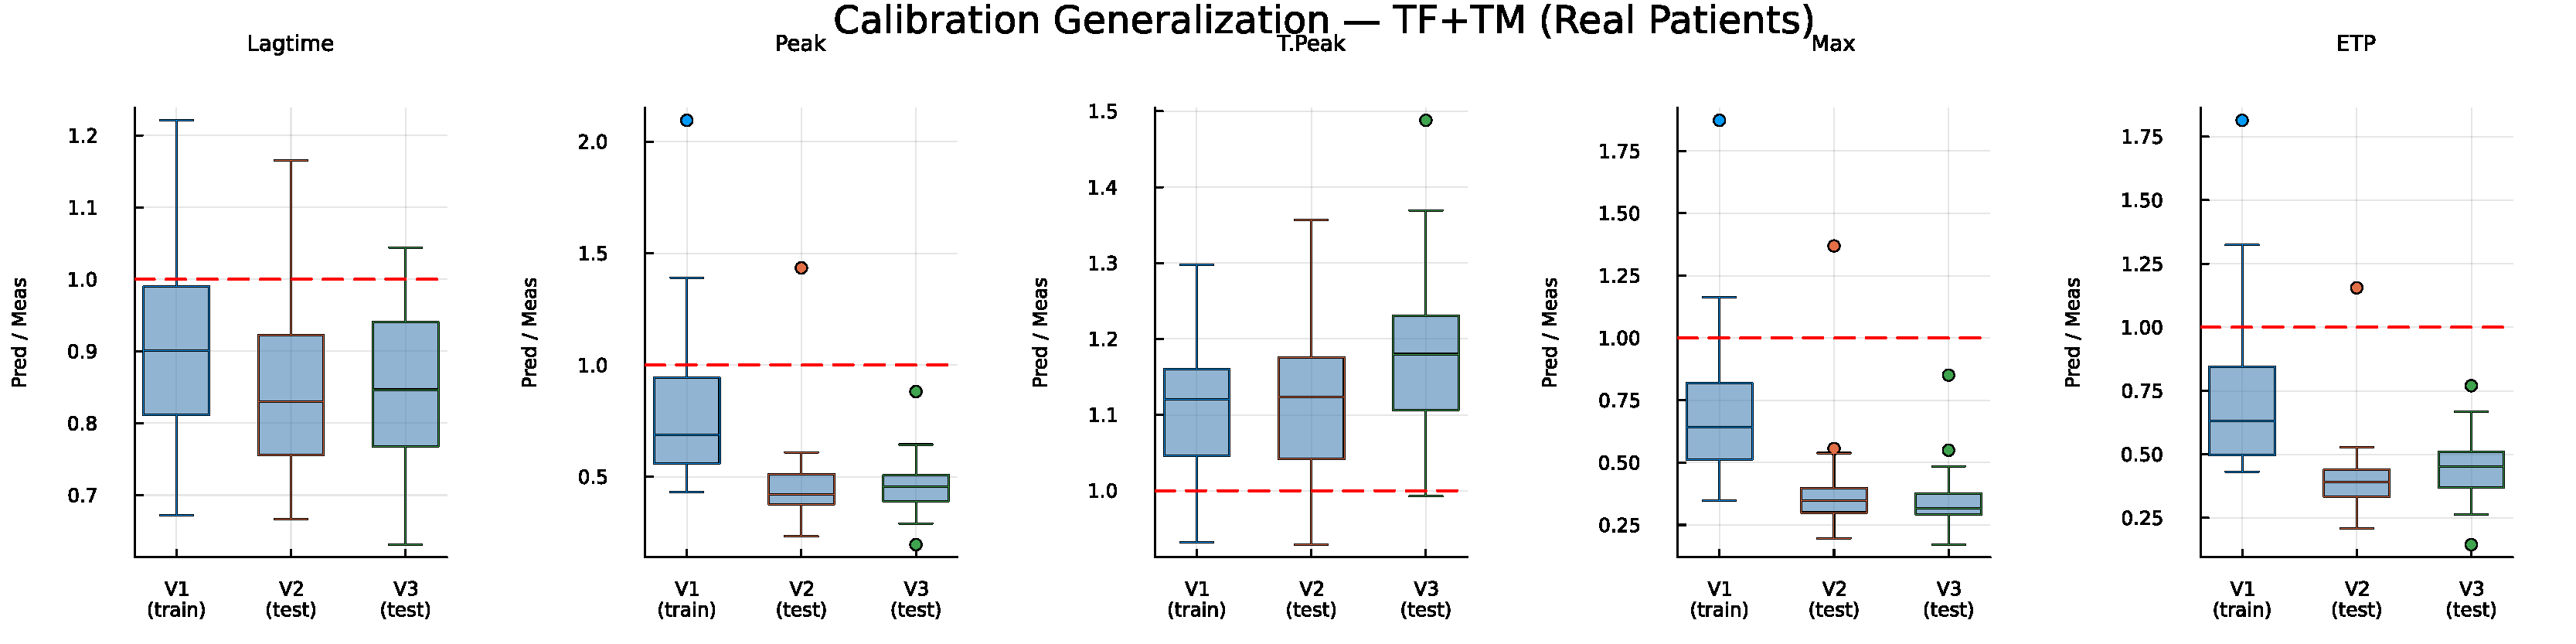
\includegraphics[width=\textwidth]{validate_mechanistic_generalization_tf_tm.pdf}
\caption{\textbf{Cross-visit calibration generalization.} Boxplots of the
ODE-predicted/dataset ratio by visit for real patients. The model was calibrated
on Visit~1 only. Top: TF-only conditions, where ratios near 1.0 at Visits~2
and~3 indicate that the calibration generalizes across pregnancy timepoints.
Bottom: TF+TM conditions, where the calibration does not generalize as well,
particularly for peak and maximum rate.}
\label{sfig:generalization}
\end{figure}

% ── Fig S7: Rank correlations (TF-only + TF+TM) ─────────────────────────
\begin{figure}[ht]
\centering
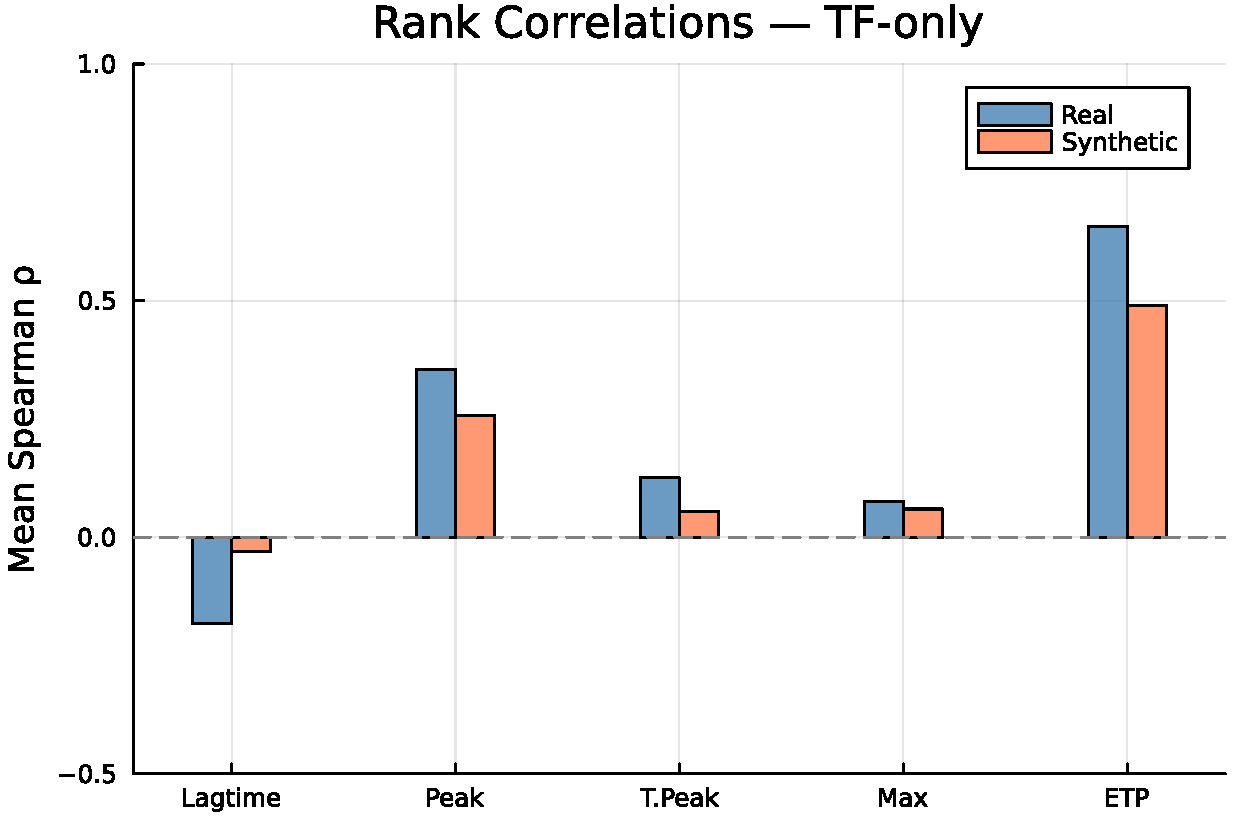
\includegraphics[width=0.48\textwidth]{validate_mechanistic_rankcorr_tf_only.pdf}
\hfill
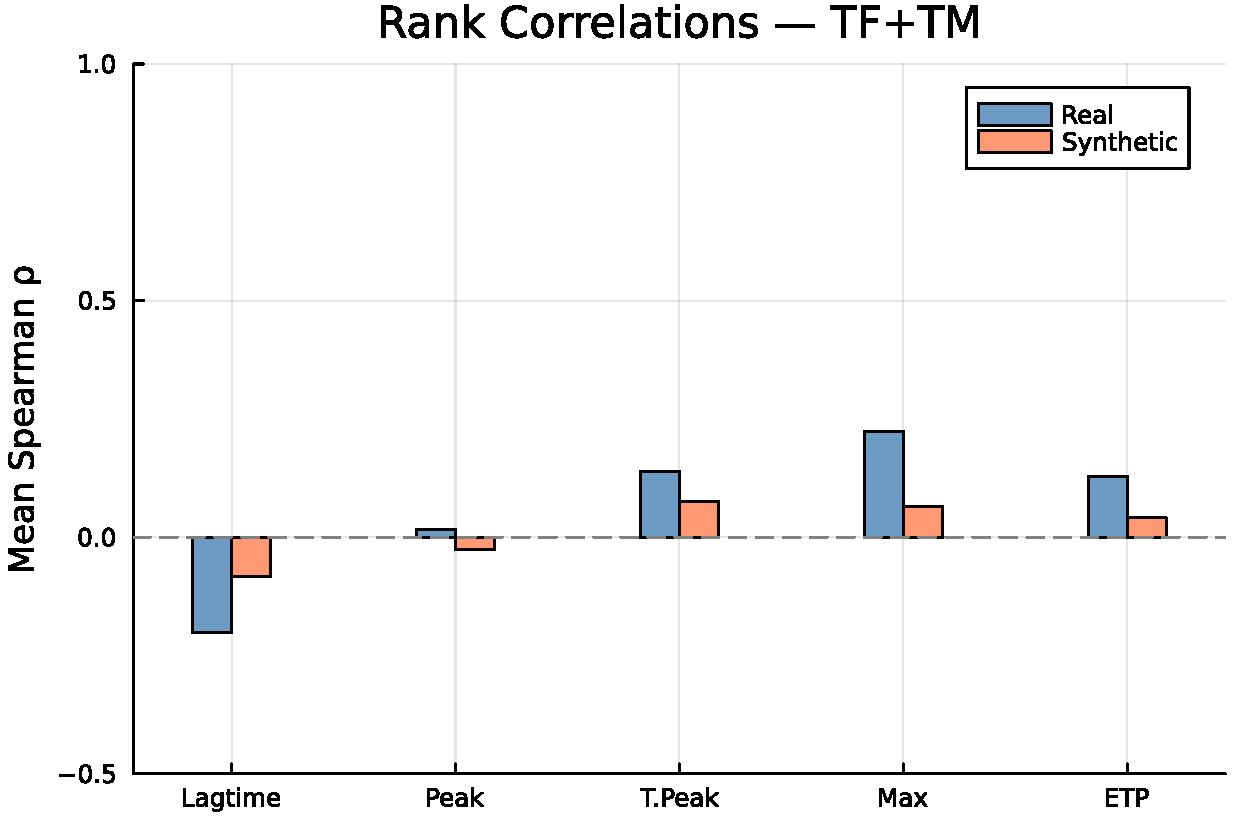
\includegraphics[width=0.48\textwidth]{validate_mechanistic_rankcorr_tf_tm.pdf}
\caption{\textbf{Spearman rank correlations between ODE-predicted and dataset
TGA features.} Left: TF-only. Right: TF+TM. ETP is the best-predicted feature
($\rho \approx 0.6$--$0.8$ for real patients under TF-only). Weak rank
correlations for other features are expected given the 5-parameter
population-level calibration.}
\label{sfig:rankcorr}
\end{figure}

% ── Fig S8: PCA projections by visit (demoted from main text per R2) ────
\begin{figure}[ht]
\centering
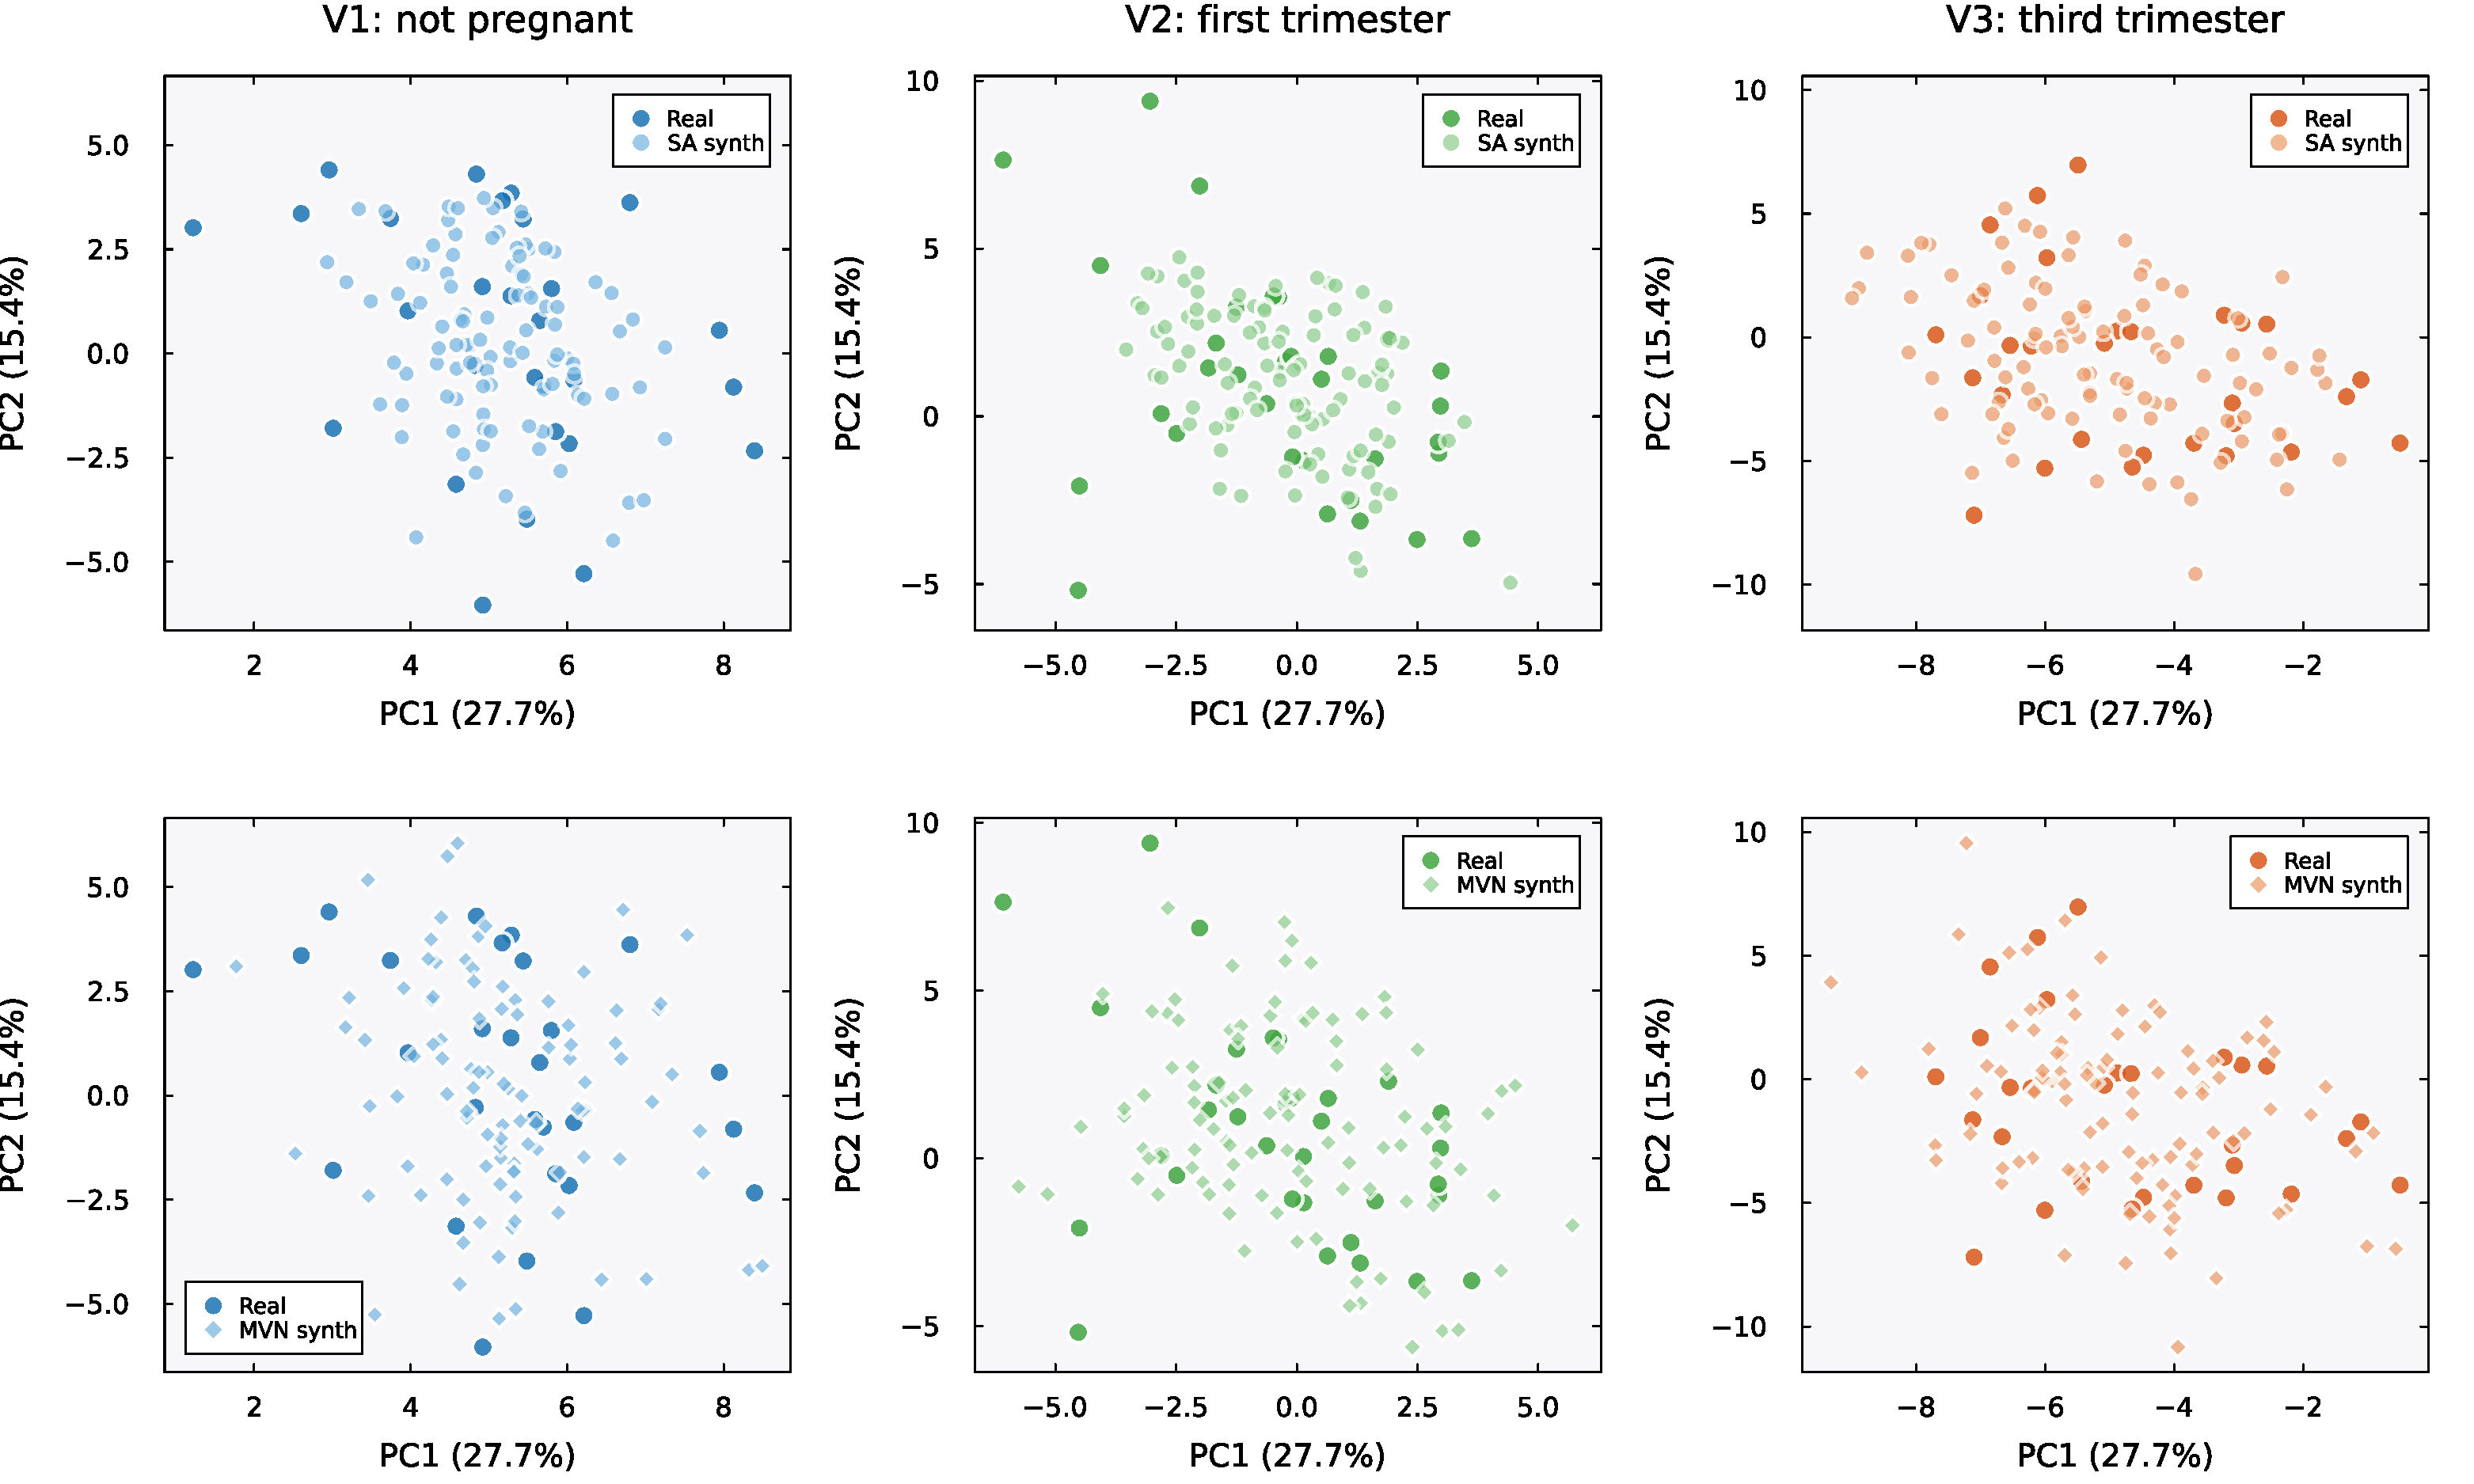
\includegraphics[width=\textwidth]{sa_vs_mvn_pca_by_visit_v2.pdf}
\caption{\textbf{PCA projections by visit: SA vs.\ MVN.} Each panel shows the
first two principal components (PC1: 27.7\% variance, PC2: 15.4\%) computed
from standardized per-visit real patient data ($K{=}23$ patients per visit,
72 features). Dark markers indicate real patients; lighter markers indicate
synthetic patients ($N{=}100$). Within each visit (column), the SA panel (top)
and MVN panel (bottom) share identical axis ranges, so the relative dispersion
of the two methods can be read against the same real data cloud. Top row:
SA-generated patients (circles)
cluster tightly around the real data cloud at all three visits. Bottom row:
MVN-generated patients (diamonds) show greater dispersion, particularly at
Visits~2 (first trimester) and~3 (third trimester), where MVN patients extend
beyond the convex hull of the real data. This excess scatter reflects the
spurious variance introduced by Ledoit--Wolf regularization of the
rank-deficient covariance (Fig.~\ref{sfig:eigenvalue-spectrum}). Colors encode visit: blue
(V1, not pregnant), green (V2, first trimester), orange (V3, third trimester).}
\label{sfig:pca-by-visit}
\end{figure}

% ── Supplementary Methods: critical inverse temperature ─────────────────
\subsection*{\rboth{Supplementary Methods: locating the critical inverse temperature}}

\rboth{The operating point $\beta^*$ was located from the attention entropy. For a candidate
$\beta$ we computed the Shannon entropy of the attention weights
$\text{softmax}(\beta\,\mhat{X}^\top\vxi)$ at $20$ probe points placed at stored patterns,
averaged those entropies, and normalized by $\log K$. The normalized curve runs from $0$ to
$1$. A value of $0$ means one pattern carries all the weight, and a value of $1$ means every
pattern carries equal weight. Sweeping $\beta$ logarithmically over $80$ values from $0.1$ to
$1000$ traces this curve from the diffuse regime into the concentrated one. We took $\beta^*$
to be the point of most negative second derivative of the normalized entropy with respect to
$\log\beta$, computed by finite differences over the sweep. That point is the sharpest bend
in the curve, and it marks where attention stops being shared across patterns and begins to
localize on one. For multiplicity-weighted sampling we repeated the same computation with the
$\log r_k$ bias included in the softmax logits. This gives a $\rho$-dependent $\beta^*(\rho)$,
because the weighting changes how quickly attention concentrates as $\beta$ grows. For random
unit-norm patterns the transition is predicted at $\beta^* = \sqrt{d}$, the theoretical
reference quoted in the main text.}

\FloatBarrier

% ── Sampling correctness and privacy diagnostics ────────────────────────
\subsection*{\rone{Sampling correctness and privacy diagnostics}}
\label{ssec:sampling-correctness}

\rone{We assessed re-identification risk directly. For every synthetic patient we
computed the distance to the closest real record (DCR) in the standardized
$216$-dimensional space and compared the synthetic-to-real distribution against the
leave-one-out real-to-real distribution. Synthetic patients sit slightly closer to the
real cohort than the real patients sit to one another, with median DCR $13.8$ against
$15.9$. We also ran a nearest-neighbor membership-inference attack, which scores each real
record by its proximity to the synthetic set over repeated random train/holdout splits. It
separated the $15$ training patients from the $8$ held-out patients with a mean AUC of $0.97$
(standard deviation $0.02$ over $40$ splits). At the published operating point the generator
therefore reproduces its training cohort closely enough to be identifiable.}

\rone{To attribute this behavior we asked whether it reflects the target distribution
$\pi(\xi)\propto\exp(-\beta E)$ or merely the sampler used to draw from it. A mixing
diagnostic showed that at $\beta^*$ the target is multimodal, with one component centered on
each of the $K{=}23$ stored patterns. It also showed that discretization bias in the Langevin
updates is negligible, with Metropolis acceptance near $0.999$
(Supplementary Fig.~\ref{sfig:mixing-diagnostic}). We then constructed a four-rung ladder
(Table~\ref{stab:sampling-ladder}, Fig.~\ref{sfig:sampling-ladder}) that holds $\beta$, the
memory, and the decoding fixed and varies only the sampler. The rungs run from the published
anchor-initialized single-endpoint scheme, to sphere initialization, to burn-in-controlled
thinned pooling, to Metropolis-adjusted sampling. Across the ladder the
membership-inference AUC stays near $0.96$ to $0.97$. The median DCR rises only from $14.0$
to $14.3$ and never reaches the real-to-real baseline of $15.9$, at a modest cost in marginal
fidelity. Proper sampling of $\pi$ does not remove the memorization. At $K{=}23$ the
memorization is a property of the distribution.}

\rone{The remaining lever is the inverse temperature. Lowering $\beta$ spreads
probability mass away from the stored patterns and should improve privacy, at the
expense of the memorization that also underlies fidelity. We swept $\beta$ across a $40$-fold
range around $\beta^*$ (Fig.~\ref{sfig:sampling-ladder}C). The sweep confirmed the trade-off
and bounded it sharply. The median DCR rises monotonically as $\beta$ falls, but it saturates
near $14.3$ and stays below the real-to-real baseline of $15.9$ even at one twentieth of
$\beta^*$. Over the same range the cross-visit covariance error grows from $0.59$ to $0.69$.
Marginal and mechanistic fidelity are insensitive to $\beta$, so the longitudinal covariance
structure bears the cost of lowering it. No inverse temperature yields a cohort that is both
as private as the real patients are from one another and faithful to their joint structure.}

\rone{Neither lever settles the question completely, because every scheme compared so far is
a finite-time Markov chain. The target itself is available in closed form. Completing the
square in Eq.~\maineqref{eq:hopfield_energy} gives Eq.~\maineqref{eq:exact_mixture}. For
unit-normalized memories $\pi_r$ is exactly the isotropic Gaussian mixture $\sum_k
q_k\,\mathcal{N}(\mathbf{m}_k,\beta^{-1}\mathbf{I})$ with $q_k = r_k/\sum_j r_j$. It can
therefore be sampled ancestrally, by drawing a component and adding isotropic noise. There is
no chain, no initialization, no burn-in and no discretization error. We generated a
protocol-matched exact cohort ($N{=}100$ at $\beta^*$, reusing the ladder's seeded magnitude
draw so that only the direction sampler differs) and evaluated it on the identical harness
(Table~\ref{stab:sampling-ladder}). Every metric falls inside the range spanned by the four
rungs: median relative error $1.68\%$, cross-visit Frobenius error $0.60$, mechanistic
overlap $0.91$, median novelty $0.50$, and median DCR $13.87$. One hundred independently
seeded exact cohorts place these quantities in narrow intervals, with median relative error
$1.40\%$ (fifth to ninety-fifth percentile $0.97$ to $1.91\%$) and median DCR $13.95$
($13.61$ to $14.39$). The agreement does not rest on a favorable seed. Over the
same $40$ train/holdout splits used for the ladder endpoints, the membership-inference AUC
under exact sampling is $0.98$, marginally above the published scheme's $0.97$. The
memorization is therefore a property of $\pi_r$ at $K{=}23$, where every stored patient is a
component center. It is not a property of any approximation used to sample it.}

\begin{table}[ht]
\centering
\small
\caption{\rone{\textbf{Sampler-correctness comparison.} Each rung holds $\beta^*$, the
memory, and the decoding fixed and varies only the direction sampler. Fidelity metrics
(median relative error, cross-visit correlation Frobenius error, mechanistic cloud
overlap, median novelty) and privacy metrics (median distance to the closest real
record, and repeated-split membership-inference AUC where evaluated) are reported per
rung. The real-to-real DCR baseline is $15.9$. The membership-inference attack was run
on the two endpoints of the ladder and on the analytic reference, over the same $40$
train/holdout splits. \emph{Exact} is not a rung. It draws ancestrally from
Eq.~\maineqref{eq:exact_mixture} with no chain, and serves as the analytic reference
for the four sampled rungs. Over $100$ independently seeded exact cohorts the median
relative error is $1.40\%$ (fifth to ninety-fifth percentile $0.97$ to $1.91\%$) and the
median DCR is $13.95$ ($13.61$ to $14.39$).}}
\label{stab:sampling-ladder}
\begin{tabular}{llcccccc}
\hline
Rung & Sampler & MRE (\%) & Cross-visit Frob. & Mech. overlap & Novelty & DCR & MIA AUC \\
\hline
V0 & anchor, endpoint & 1.31 & 0.65 & 0.89 & 0.51 & 13.97 & 0.97 \\
V1 & sphere init      & 1.53 & 0.57 & 0.89 & 0.50 & 13.96 & n/a  \\
V2 & pooled ULA       & 2.02 & 0.59 & 0.88 & 0.50 & 14.15 & n/a  \\
V3 & pooled MALA      & 1.89 & 0.62 & 0.92 & 0.52 & 14.33 & 0.96 \\
\hline
\rone{Exact} & \rone{analytic ancestral} & \rone{1.68} & \rone{0.60} & \rone{0.91} & \rone{0.50} & \rone{13.87} & \rone{0.98} \\
\hline
\end{tabular}
\end{table}

\begin{figure}[ht]
\centering
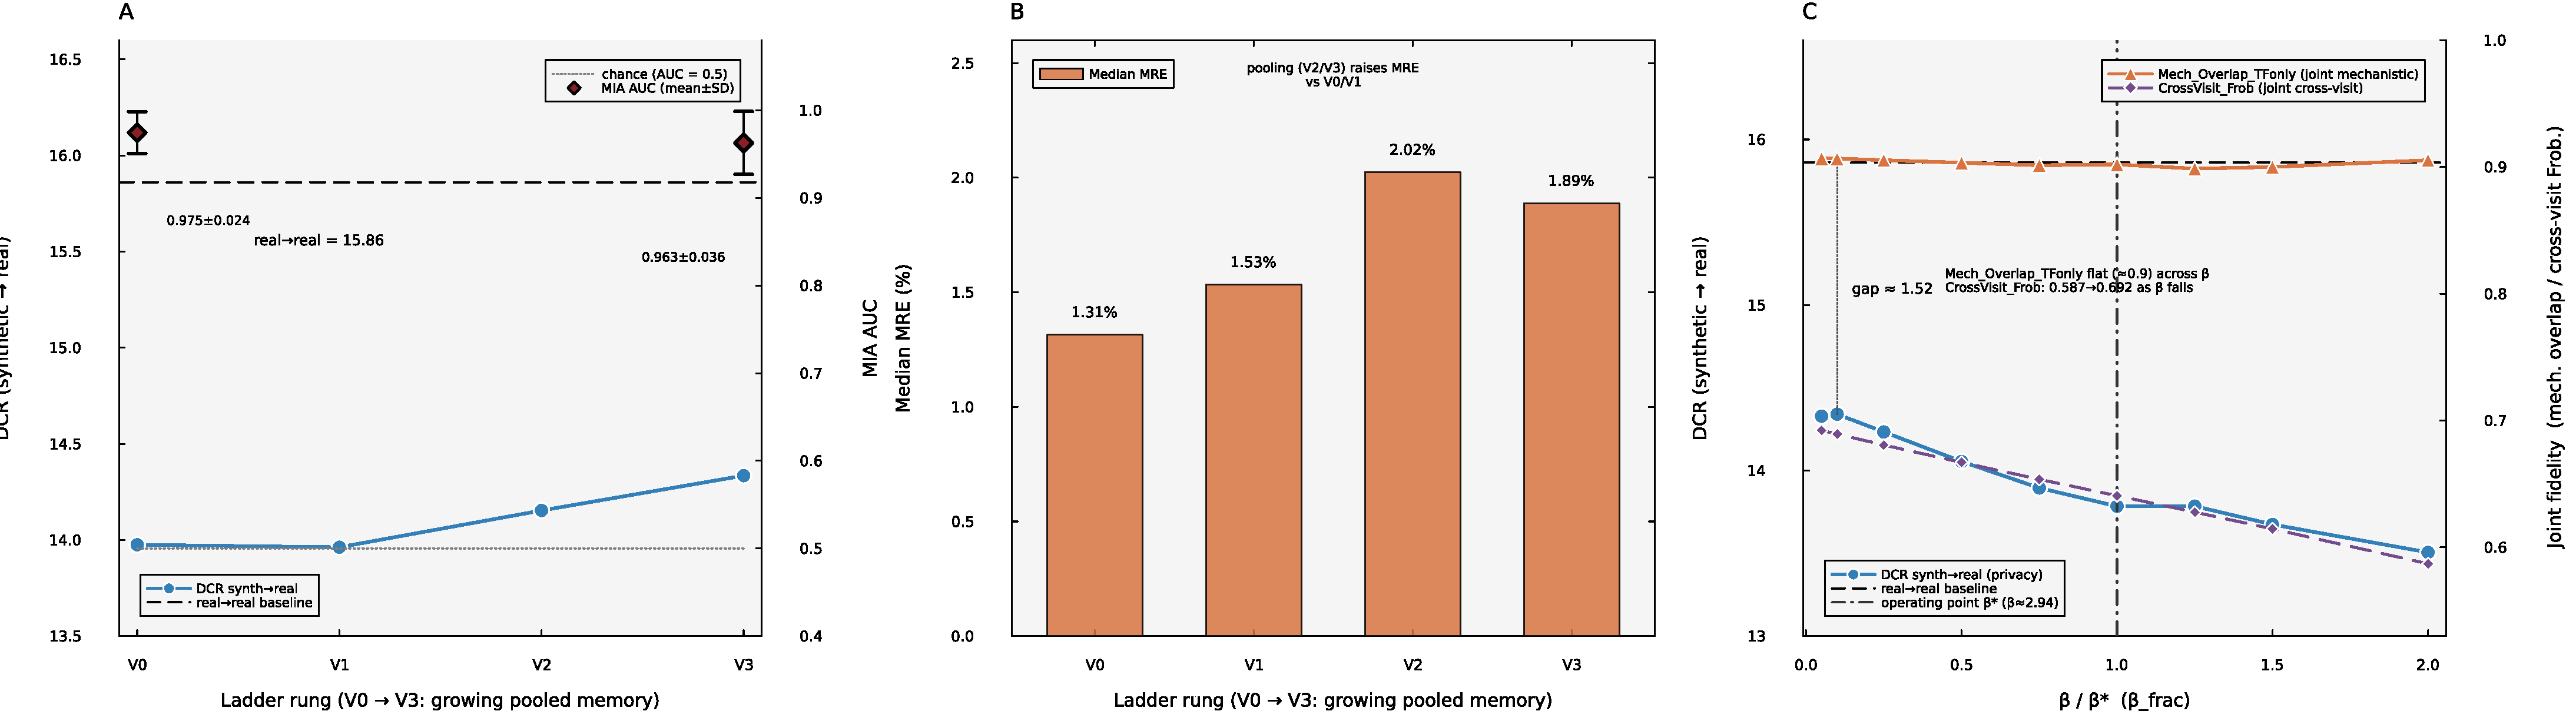
\includegraphics[width=\textwidth]{mcmc_ladder.pdf}
\caption{\rone{\textbf{Sampling correctness and the memorization/privacy relationship.}
(A) Across the V0 to V3 ladder the distance to the closest real record (DCR, left axis)
rises only slightly and stays below the real-to-real baseline, while the
membership-inference AUC (right axis) remains near $0.96$ to $0.97$. (B) The fidelity
cost of multi-chain pooling, as median relative error. (C) The inverse temperature swept
across a $40$-fold range around the operating point $\beta^*$. The DCR (privacy, left axis)
rises as $\beta$ falls but never reaches the real-to-real baseline. The cross-visit
covariance error (right axis) grows, and the mechanistic overlap stays flat.}}
\label{sfig:sampling-ladder}
\end{figure}

\begin{figure}[ht]
\centering
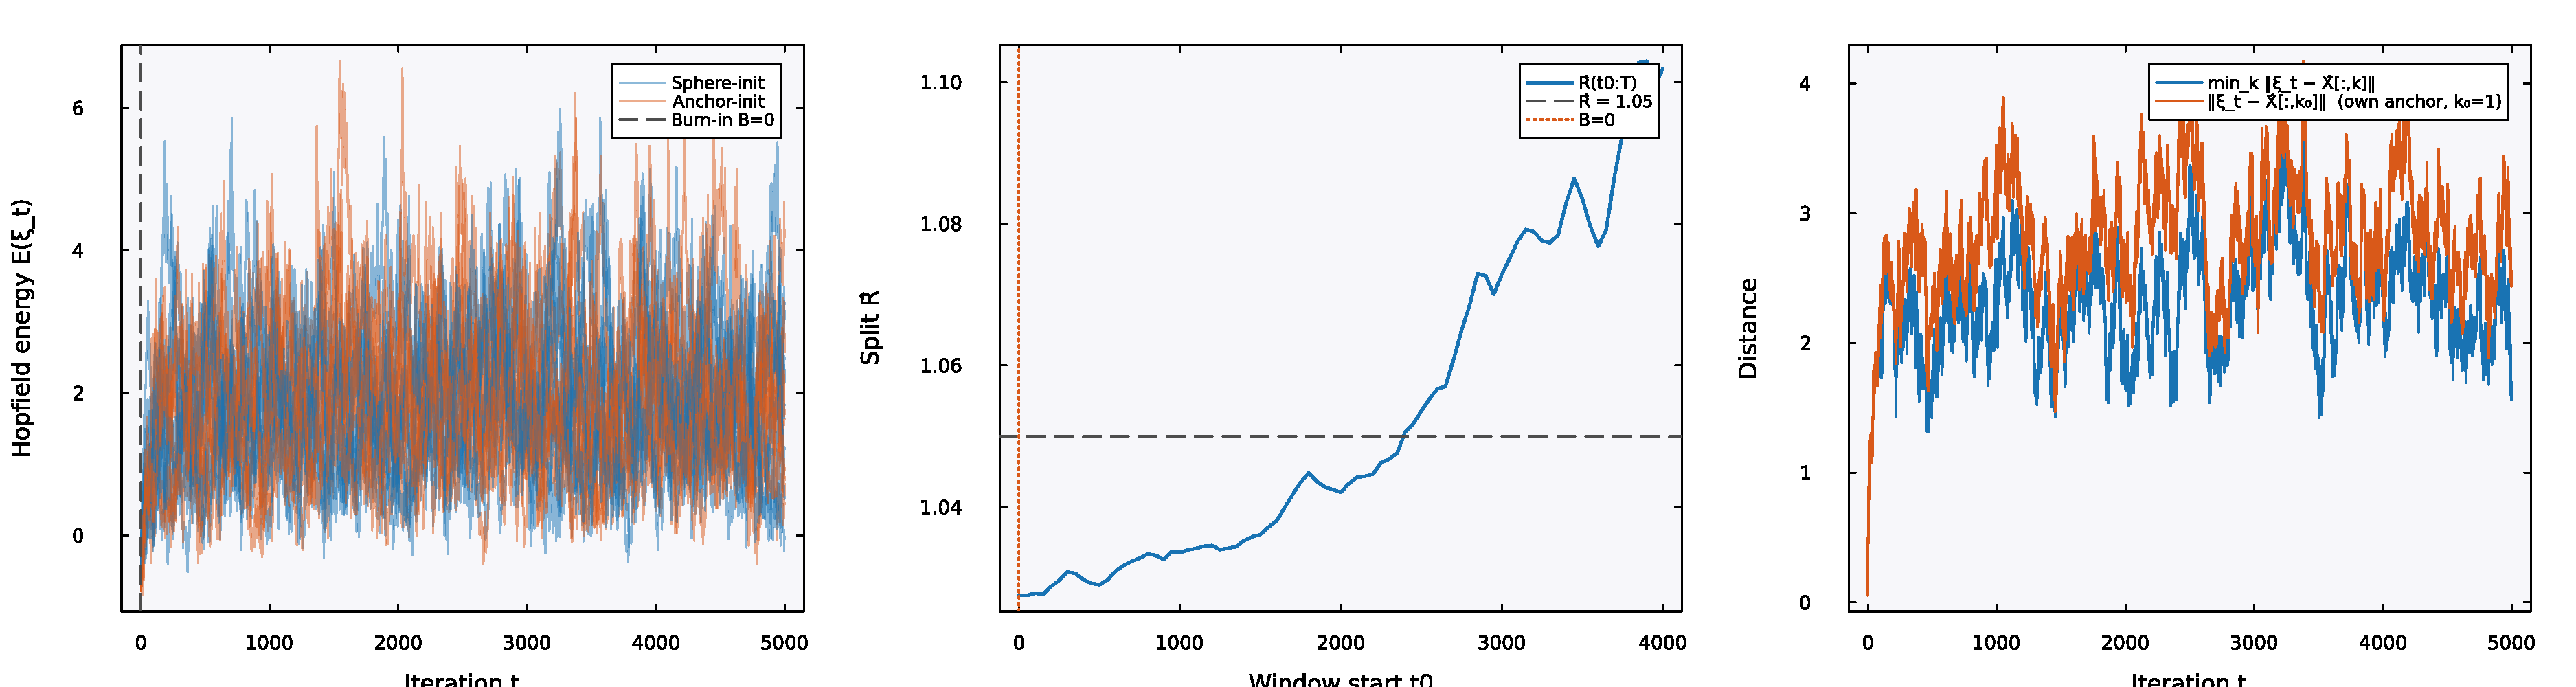
\includegraphics[width=\textwidth]{mcmc_mixing_diagnostic.pdf}
\caption{\rone{\textbf{Mixing diagnostic at $\beta^*$.} Energy traces, the between-chain
$\hat{R}$ statistic, and the anchor-distance trajectory for sphere-initialized Langevin
chains. The target distribution at $\beta^*$ is multimodal, with one component centered on
each stored pattern. Metropolis acceptance near $0.999$ indicates negligible discretization
bias.}}
\label{sfig:mixing-diagnostic}
\end{figure}


\end{document}
